% \begin{savequote}[8cm]
% \textlatin{Pulchra es, suus 'verum,}
% 
% You're beautiful, it's true.
%   \qauthor{--- James Blunt's \textit{You're Beautiful}}
% \end{savequote}

\chapter{\label{ch:3-TORCH}TORCH}

\minitoc

\section{Introduction}
% The \DstrDecay\ decay, described in Sec. \ref{sec_Physics_Background} and shown in \fig{fig_SlowPMom}, is an example of a low-momentum background in which improved PID capabilities of the LHCb detector could provide significant added value.
% Currently the LHCb PID system relies upon the RICH detectors and does not perform as well in the low momentum region (defined to be $p < 10$\GeVMom) as it does at higher values \cite{Papanestis_2017}. The TORCH detector is a proposed upgrade to LHCb intended to provide efficient PID over the while momentum range \cite{vanDijk_2014}.

The TORCH (Time Of interally Reflected CHerenkov light) detector measures Time of Flight (ToF) to perform PID. Particles of the same momentum but differing mass will take different times to cover the same distance, given by
\begin{equation}
t = \frac{x}{c} \sqrt{1 + \left(\frac{mc}{p}\right)^{2}}.
\end{equation}
TORCH is designed to exploit this time of flight difference to distinguish between pions, kaons, and protons \cite{vanDijk_2016}. Using the Taylor expansion for $\sqrt{1+x}$, the time of flight difference for two species can be written as
\begin{equation}
\Delta t_{1,2} \approx \frac{x}{c}\frac{1}{2p^{2}} (m_{1}^{2} - m_{2}^{2}).
\end{equation}

The TORCH detector consists of adjacent plates of $1\,\rm{mm}$ thick quartz which cover the area of LHCb perpendicular to the beamline, situated approximately $9.5\,\rm{m}$ from the interaction region \cite{vanDijk_2016}. 
%, as shown in \fig{fig_Plates_Layout}. 
When a charged particle passes through one of these plates, Cherenkov photons are generated. These photons are trapped by Total Internal Reflection (TIR) and travel  to the top of the plate, where they are focused onto an array of Micro-Channel Plate (MCP) detectors.  MCPs are able to detect single photons with excellent resolution, typically $50\,\rm{ps}$, thus making them an idea choice for TORCH. The setup of the focusing optics is shown in \fig{fig:FocusingBlock}. The optics map the photon angle to position in the focal plane, allowing the angle of arrival to be determined. This is essential for the performance of TORCH as it allows chromatic dispersion to be accounted for in the reconstruction.

\begin{figure}
\centering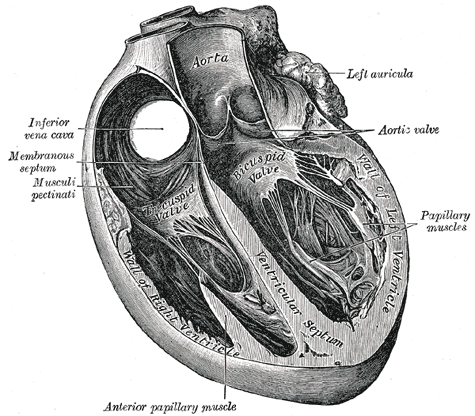
\includegraphics[width=0.7\textwidth]{figures/sample/Gray498.png} 
\caption[Four-chamber illustration of the human heart.]{Four-chamber illustration of the human heart.  Clockwise from upper-left: right atrium, left atrium, left ventricle, right ventricle.}
\label{fig:FocusingBlock}\end{figure}

\section{Design of TORCH}

\subsection{Optics}
Radiator Plate.

Focusing Block.

Glue used to optically connect them.

\subsection{TORCH MCPs}
Overview of MCP required specs and design.

Difference in two Phase 3 tubes used in testbeam.

\subsection{Readout Electronics \& DAQ}
Overview of readout electronics chain.

\section{Testbeam Setup}
Introduce Testbeam setup.

\subsection{Overview}
Overview of testbeam setup, inc. diagram of layout. Introduce two testbeam periods and say the infrastructure was the same, but mini-TORCH was modified between the two.

\subsection{Mini-TORCH}
Description of mini-TORCH in reference to overall TORCH design.

\subsection{Timing Stations}
Description of timing stations, inc. borosilicate fingers and scintillators.

\subsection{Beam Telescope}
Description of beam telescope.

\subsection{Cherenkov Counters}
Description of Cherenkov Counters.

\section{Testbeam Analysis}
Introduction to analysis. Purpose is to measure single photon time resolution of TORCH. Reminder of the two Testbeam periods.

\subsection{INL Correction}
Describe INL correction and how its performed.

\subsection{Time of flight difference}
Show Time of Flight difference for each testbeam and energy. Show INL improves the resolution and show comparison with the Cherenkov counter decision.

\subsection{Beam Momentum Measurements}
Give beam momentum measurements for each period of beam energy.

\subsection{Clustering}
Describe clustering algorithm and any changes between the two testbeams.

\subsection{Timewalk Correction}
Describe timewalk correction, but don't need to go into detail. Make explicit time walk correction was generated elsewhere.

\subsection{Beam Telescope Integration}
Describe how beam telescope is integrated into the analysis.

\subsection{Time of Propagation Correction}
Go through derivation of ToP correction and its application using the telescope.

\subsection{Time Projections}
Give time projection plots for the two analyses.

\subsection{Photon Reconstruction}
Details of the photon reconstruction algorithms.

\subsection{Data-driven Alignment}
Describe the procedure and method of carrying out the data-driven alignment.

\subsection{Time Reference Time Resolution}
The time resolution of TORCH is measured with respect to the time reference provided by the second time reference station. As such, it is necessary to measure the time resolution of the time reference so that it can be disentangled from the individual photon resolution of TORCH. The testbeam infrastructure includes two time reference stations of identical design, and so these can be used to benchmark each other.

Each timing station consists of two parts, a Cherenkov radiator connected to a single channel MCP which provides the time reference, and a pair of cross scintillators for which a signal can be required (see Section XXX). 
Requiring a scintillator signal improves the time resolution of station by narrowing the cross-section of Cherenkov radiator which the beam strikes. This allows different measurement conditions to be constructed, and through comparison of the time resolution with and without scintillator signals, the time resolution of the timing stations can be determined.

Three sets of measurement conditions are used to measure the timing station time resolution:
\begin{enumerate}
\item Both timing stations require scintillator signals.
\item Scintillator signal required for downstream station but not for upstream.
\item Neither timing station requires a scintillator signal.
\end{enumerate}
A forth set of conditions is possible, requiring a scintillator signal in the upstream station but not the downstream. This significantly reduces the rate of data taking however, and so the other three sets of conditions were considered preferable.

The time resolution measurement makes three assumptions.
\begin{enumerate}
\item The intrinsic time resolution of both timing stations is the same
\item Any observed difference is due to signal degradation in the cable from the upstream station.
\item The amount of degradation is independent of requiring a scintillator signal.
\end{enumerate}

The combined resolution of the two timing stations can be measured using the time of flight distribution for protons and pions. The width of each given peak is the combination of the two stations added in quadrature,
\begin{equation}
\label{eqn:TORCH_ToFResolution}
\sigma_{ToF}^{2} = \sigma_{upstream}^{2} + \sigma_{downstream}^{2},
\end{equation}
where $\sigma_{ToF}$ is the width of the proton/pion peak, $\sigma_{upstream}$ is the resolution of the upstream timing station, and $\sigma_{downstream}$ is the resolution of the downstream timing station (Note, both $\sigma_{upstream}$ and $\sigma_{downstream}$ refer to the resolution seen after the signals are injected through the TORCH electronics, not the intrinsic resolutions).

From equation \ref{eqn:TORCH_ToFResolution}, three resolution equations can be written,
\begin{equation}
\label{eqn:TORCH_ToFResolution_CondA}
\sigma_{both}^{2} = (\sigma_{upstream}^{\prime} )^{2} + (\sigma_{downstream}^{\prime} )^{2},
\end{equation}
\begin{equation}
\label{eqn:TORCH_ToFResolution_CondB}
\sigma_{down\,only}^{2} = (\sigma_{upstream} )^{2} + (\sigma_{downstream}^{\prime} )^{2},
\end{equation}
\begin{equation}
\label{eqn:TORCH_ToFResolution_CondC}
\sigma_{neither}^{2} = (\sigma_{upstream} )^{2} + (\sigma_{downstream} )^{2},
\end{equation}
where a prime denotes the requirement of a scintillator signal for that timing station.

To account for signal degradation between the two stations, a factor $\phi$ is introduced, providing a link between the two station resolutions,
\begin{equation}
\label{eqn:TORCH_TimeRefRes_T1toT2}
\sigma_{downstream} = \phi\sigma_{upstream}
\end{equation}
and 
\begin{equation}
\label{eqn:TORCH_TimeRefRes_T1PrimetoT2Prime}
\sigma_{downstream}^{\prime} = \phi\sigma_{upstream}^{\prime}.
\end{equation}

Using equations \ref{eqn:TORCH_ToFResolution_CondA} to \ref{eqn:TORCH_TimeRefRes_T1PrimetoT2Prime}, the resolution of each station and the factor $\phi$ can be determined from the with of the proton/pion peak through the following:
\begin{equation}
\phi^{2} = \frac{\sigma_{both}^{2} - \sigma_{down\,only}^{2}}{\sigma_{down\,only}^{2} - \sigma_{neither}^{2}},
\end{equation}
\begin{equation}
(\sigma_{downstream}^{\prime} )^{2} = \frac{\sigma_{both}^{2} }{1 + \phi^{2}},
\end{equation}
and
\begin{equation}
(\sigma_{downstream})^{2} = \frac{\sigma_{neither}^{2} }{1 + \phi^{2}}.
\end{equation}

The resolutions measured for each set of conditions are given in Table \ref{tab:TORCH_TimeRefRes_PeakWidths}, and the derived time resolutions in Table \ref{tab:TORCH_TimeRefRes_Results}.

\begin{table}[h]
\centering
\begin{tabular}{|c|c|}
\hline
Conditions & Pion Peak Width \\ \hline
Both & $91\pm1\,\rm{ps}$ \\
Down only & $124\pm1\,\rm{ps}$ \\
Neither & $131.6\pm0.3\,\rm{ps}$ \\ \hline
\end{tabular}
\caption{Blah.}
\label{tab:TORCH_TimeRefRes_PeakWidths}
\end{table}


\begin{table}[h]
\centering
\begin{tabular}{|c|c|}
\hline
Variable & Value \\ \hline
$\phi$ & $91\pm1\,\rm{ps}$ \\
$\sigma_{downstream}^{\prime}$ & $42 \pm 3 \,\rm{ps}$ \\
$\sigma_{downstream}$ & $61 \pm 4 \,\rm{ps}$ \\ \hline
\end{tabular}
\caption{Blah.}
\label{tab:TORCH_TimeRefRes_Results}
\end{table}


\subsection{TORCH Time Resolution}
Final Time Resolution Measurement.

